\documentclass[runningheads,a4paper]{llncs}

\usepackage{xeCJK}
\setCJKmainfont[BoldFont=STHeiti, ItalicFont=STKaiti]{STSong}
\setCJKsansfont[BoldFont=STHeiti]
\setCJKmonofont{STFangsong}

%\usepackage[BoldFont,SlantFont,CJKchecksingle]{xeCJK}
%\setCJKmainfont[BoldFont=SimHei]{SimSun}
%\setCJKmonofont{SimSun}% 设置缺省中文字体
%\usepackage{CJKutf8}

\usepackage{amssymb}
\usepackage{graphicx}
\usepackage{url}
\usepackage{color}
%\usepackage{CJK}

\usepackage{url}
\usepackage[ruled]{algorithm2e}
\usepackage{amsmath}
\usepackage{graphicx}
\usepackage{enumerate}

\urldef{\mailthu}\path|{lmy13@}tsinghua.edu.cn|
\urldef{\mailsy}\path|{fantasysy@}sina.com|
\newcommand{\keywords}[1]{\par\addvspace\baselineskip\noindent\keywordname\enspace\ignorespaces#1}
\newcommand{\para}[1]{\vspace{0.1cm}\noindent\textbf{#1}}

\begin{document}
%\begin{CJK*}{UTF8}{simsun}
\mainmatter

\title{Building Large-Scale Cross-lingual Knowledge Base from Multi-Encyclopedia}
\titlerunning{Bilingual Knowledge Base}
\author{Mingyang Li$^\dag$ \and Yao Shi$^\dag$ \and Zhigang Wang$^\dag$}
\authorrunning{Mingyang Li et.al}

\institute{$^\dag$Tsinghua National Laboratory for Information Science and Technology,\\
Department of Computer Science and Technology,\\
Tsinghua University, Beijing 100084, China\\
\mailthu\\
\mailsy\\
}

\maketitle

\begin{abstract}
    Abstract Text

\keywords{Knowledge Base, Semantic Web, Ontology, Cross-lingual}
\end{abstract}

\section{Introduction}
With Linked Open Data(LOD) developing recent years, an increasing number of knowledge bases are generated for information sharing. Large-scale knowledge bases in LOD project, such as DBpedia\cite{mendes2012dbpedia}, YAGO\cite{mahdisoltani2014yago3} and Freebase\cite{bollacker2008freebase} are often used for information extraction\cite{dutta2013integrating}, entity linking\cite{shen2012linden}, recommendation\cite{passant2010dbrec,fernandez2011generic,kaminskas2012knowledge}and many other applications. These knowledge bases are not only cross-domain but also multilingual, which is benefit for global knowledge sharing.  

 The nucleus of LOD DBpedia extracts structured information from Wikipedia and has already contained approximately 38.3 million things. Now DBpedia provides 124 versions of non-English language including Chinese. However, there are only XXX instances and 11 classes in Chinese. Compared with the 4.58 million things in English, the quality of Chinese information is obviously insufficient for further research and application.

A cross-lingual knowledge base can effectively promote global knowledge sharing, understanding and expanding. However, to build an available knowledge base, some problems must be addressed: (1) The imbalanced size of different language sources leads to less entities. Comparing the number of articles in English Wikipedia with those in Chinese Wikipedia, which are 5 million and 800 thousand separately, it's obvious that to structure a knowledge base in Chinese with Wikipedia is more challenging. (2) The number of existing cross-lingual links in Wikipedia accounts for a low proportion, which affects the quality of a bilingual knowledge base. Especially when there are scarce evident links in properties. Statistically, only XX thousand cross-lingual links can be found between English and Chinese articles. (3) The large but not rigorous category system in Wikipedia causes incorrect semantic relations in taxonomy. For example,\textcolor{red}{example}

%In Semantic Web, a large-scale multilingual knowledge base can help …

%Thus it’s significant to build a Chinese-English knowledge base and benefit from it.

Currently, there are several massive knowledge encyclopedias in Chinese, including Hudong Baike and Baidu Baike. To solve the imbalance problem, we utilize such separated sources to enrich our Chinese information. In this paper, we propose an approach to integrate four resources, which are English Wikipedia, Chinese Wikipedia, Hudong Baike and Baidu Baike, into one cross-lingual knowledge base, which contains XXX concepts, XXX instances and XXX properties. To get a more available result, we also make judgement on the relations among concepts and instances. At last, a SPARQL endpoint is provided to access to the knowledge base. Specifically, our work makes the following contributions:
\begin{itemize}
  \item We propose a method to build a Chinese-English cross-lingual knowledge base combining multi-encyclopedias. Among them, two  Chinese encyclopedias are utilized to help balance and enrich information in two languages.
  \item We extend the cross-lingual link set by employing a cross-lingual knowledge linking discovery approach for concept and instance, and analyzing templates in Wikipedia for property.
  \item We prune the original taxonomy, which is extracted from encyclopedia category system, to retrieve more precise SubClassOf and InstanceOf relations in ontology.
  \item Both website and SPARQL endpoint is provided for public query operations over our knowledge base.
\end{itemize}

The rest of the paper is organized as follows. Section \ref{sec:pd} introduces the four involved encyclopedias. Besides, the procedure are formalized in this section. Section \ref{sec:dp} presents the extraction approach in concept, instance and property level. Section \ref{sec:clkbb} describes the procedure of building a knowledge base using extracted result. Section \ref{sec:result} shows the data situation of established knowledge base. Section \ref{sec:work} induces related work about this paper. Section \ref{sec:con} gives the conclusion.

\section{Problem Definition}
\label{sec:pd}
In this section, we firstly introduce the four encyclopedias used to build and enrich our knowledge base. Then we give some related definitions to formalize our ontology model. 

\subsection{Encyclopedias}
\label{sec:encyclopedias}
\subsubsection{Wikipedia}
Nowadays, Wikipedia is the largest data store of human knowledge. It was launched in 2001 and has hold over 35 million articles in 288 languages by 2015. Out of these, English articles contribute most. The imbalance of different language articles makes ontologies based on Wikipedia-only behave badly in cross-lingual aspect. Thus, more Chinese encyclopedias are necessary to enrich Chinese source.

Among the large-scale monolingual Chinese encyclopedias currently, Baidu Baike and Hudong Baike are the most content-rich. Hudong Baike was founded in 2005 and contains more than 12 million articles with about 9 million experts' contribution until 2015. Meanwhile, Baidu Baike maintains more than 11 million articles. 

Articles from the four sources are similar in structure. Usually they provide two important elements with potential semantic information, category taxonomy and articles. A taxonomy presents the relations between categories. Usually a category has sub-categories and super-categories. Fig.\ref{fig:hudong-taxonomy} shows a screenshot of Hudong Taxonomy. An article describes an entity with rich information created and modified by several verified editors. Besides, an article may belong to one or more categories. The article content as well as the relation between an article and its belonged categories both help enormously when constructing a knowledge base. In general, there are five elements can be exploited in each article page:
\begin{figure}
    \centering
    \begin{minipage}[t]{0.8\textwidth}
        \centerline{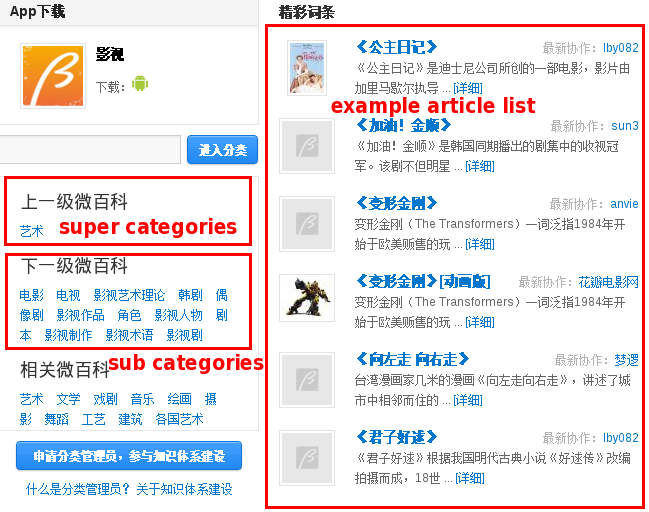
\includegraphics[width=0.8\columnwidth]{fig/hudong-taxonomy2}}
        \caption{Taxonomy in Hudong}
        \label{fig:hudong-taxonomy}
    \end{minipage}%
\end{figure}
\begin{itemize}
  \item Title: A Title is the label of an entity, which is unique so that it can be used to distinguish entities.
  \item Abstract: An abstract is a brief summary of the entity. It's always the first paragraph of an article. 
  \item Infobox: Most of articles contain infobox. An infobox maintains structured data which are subject-attribute-value triples formalized as a table. Information in this table includes important properties of an entity.
  \item Links: Links are entries to other articles within the encyclopedia. They lead readers to reference articles. Actually, they represent the relations between the current article and other articles.
  \item Category: The categories that an article belongs to are usually listed at the bottom of article page, shown as tags. An article belongs to one or more categories.
\end{itemize}

Fig. \ref{fig:interstellar} shows a snap of an article in Chinese Wikipedia.
\begin{figure}[ht]
    \centerline{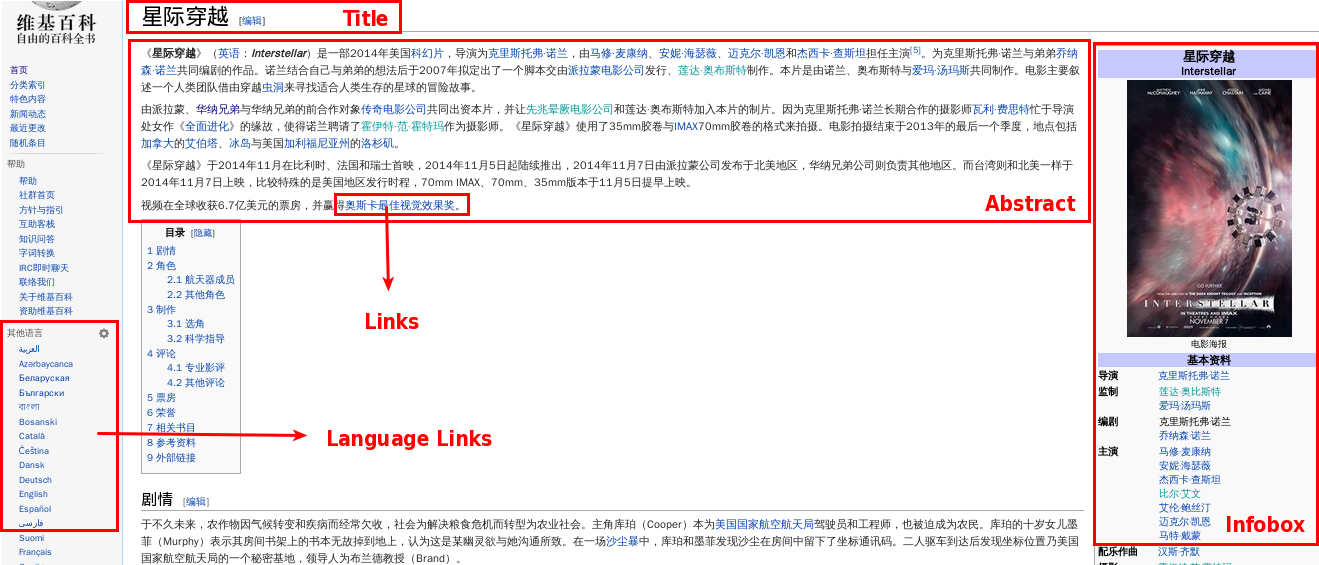
\includegraphics[width=1\columnwidth]{fig/interstellar}}
    \caption{A snap of Interstellar(Film) article in Chinese Wikipedia}
    \label{fig:interstellar}
\end{figure}%

Notably, articles in Wikipedia follow templates specified by Wikipedia when being editted. A template defines items that a group of article should fill. Besides, infoboxes are generated based on templates too. For example, The infobox in film 星际穿越(Interstellar) is edited according to the Template \emph{Infobox film}, which maintains a property set of films.

Moreover, in Wikipedia, some article pages have language links which help readers switch to other language-version within the same article. Fig. \ref{fig:interstellar}shows language links of \emph{Interstellar} on the right column of the Wikipedia page. Taking advantage of manually established language links, we can generate an initial cross-lingual ontology.

\subsection{Definitions}
\label{sec:definition}
Here we list some definitions involved in the later sections:

\textbf{Definition 1:} An encyclopedia is considered as a collection of articles, category system, which can be defined as: $W = <A,C>$, where A denotes articles, C denotes categories in W.

According to Section \ref{sec:encyclopedias}, the elements of each article $a$ can be defined as follow:
\begin{equation}
    a = <Ti(a),Ab(a),Li(a),In(a),C(a),U(a)>
\end{equation}
where $Ti(a),Ab(a),Li(a),In(a),C(a),U(a)$ denotes title, abstract, links, infobox, category tags, url of article $a$.

The topic described by $a$ is defined as Entity$e$. Ariticles from different sources may talk about the same entity. In such a situation, we say the articles are linked. 

\textbf{Definition 2:} As to an article $a$ containing multi-language content in Wikipedia, $L_{e}$ and $L_{z}$ denotes its article links, usually titles, in English and Chinese separately. Thus, to a $cl$ in $CL$, $cl(a) = <L_{e}(a), L_{z}(a)>$

\textbf{Definition 3:} An Infobox $In(a)$ in an article contains a set of attribute-value pairs {$p_{1}$, $p_{2}$,...}. In Wikipedia, an infobox is usually edited based on an appropriate infobox template recommended by Wikipedia, which here we denote as $T(a)$. Templates specify certain attributes, which are usually different from those displayed on the webpage. Thus, we define an attribute-value pair as a triple $p=<tl,dl,v>$, where $tl$ is attribute label in template, $dl$ is displayed label in web page and $v$ is the corresponding value.

\textbf{Definition 4:} An ontology is a formal specification of a group of entitie. In our work, an ontology is described as a 6-tuple:
\begin{equation}
    O = <C,I,P,H^C,H^I,H^P>
\end{equation}
where $C$, $I$, $P$ are the sets of concepts, instances, and properties, respectively. $H^C$, $H^I$, $H^P$ represents the hierarchical relationships of concept-concept, concept-instance, instance-property. A Taxonomy$T$ is comprised by $H^C$ and $H^I$, which seperately repesent \emph{SubClassOf} and \emph{InstanceOf} relations.

\subsection{Cross-lingual Knowledge Base Building}
A cross-lingual knowledge base is a database conform to a cross-lingual ontology. Taking advantage of language links in $CL$, several mono-ontologies generated from various sources can be merge into one cross-lingual ontology.  Thus a knowledge base can be defined as:
\begin{equation}
    KB = <O_{i}, CL>
\end{equation}
where $O_{i}$ denotes the ith mono-ontology, CL represents the cross-lingual link set.
We build the cross-lingual ontology according to the procedure in Fig. \ref{fig:procedure}
\begin{figure}[ht]
    \centerline{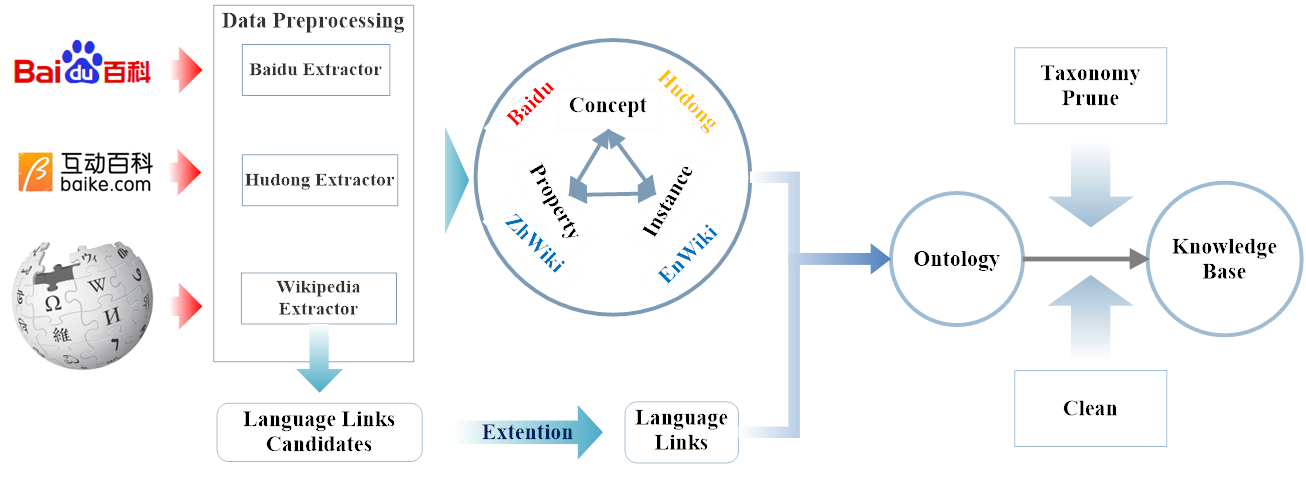
\includegraphics[width=1\columnwidth]{fig/procedure}}
    \caption{Procedure of building our cross-lingual knowledge base}
    \label{fig:procedure}
\end{figure}%
We extract information from four sources, Baidu Baike, Hudong Baike, Chinese Wikipedia and English Wikipedia. Considering the different data format of each source, that is, html code page of Baidu and Hudong with different layout, and XML format of Wikipedia dump file, various extractors should be employed. After data parsing, we get four datasets with concept lists, instance lists, property lists and their relations of each source. Meanwhile, an initial Chinese-English language-link set is generated, which will be increased by employing a link-discovery method to obtain a larger one. Using the extended language links, we combine the four datasets into one. At last, going through the procedure of taxonomy pruning and data-cleaning, we get a final knowledge base with higher accuracy.

\section{Semantic Data Extraction}
\label{sec:dp}
We prepare data for the knowledge base by a series of extracting operations. During this stage, our goal is to get a structured dataset including concepts, which are extracted from category taxonomy; instances, which are defined according to articles, and properties based on both infobox and templates assistant. We will describe the extraction approach in detail below.

\subsection{Concept Extraction}
\label{sec:ce}
A concept is defined as a type of similar instances. For example, the concept of instance \emph{Interstellar} is \emph{Movie}. In general, a concept has super classes and sub classes, which means it has \emph{SubClassOf} relation with other classes. Concepts comprise a taxonomy which presents a backbone of an ontology.

In an encyclopedia, a category groups several articles and also has super-categories and sub-categories, just like concept does. Therefore we can extract concepts based on existing category system.

However, the whole taxonomy can not directly transform from category system because of the following problems:
\begin{itemize}
    \item There are auxiliary categories in Wikipedia, which help arrange specific articles or category pages. For example, \emph{Lists of artists} or \emph{Food templates}.
    %s\item Some sub-category links in the category system maybe inconsistent. Some categories may contain itself as sub-category, or contain sub-category that also be the super-category of it. As Fig. \ref{fig:category-mistakes} shows: In Hudong, the sub-category of 国家元首(Head of State) contains itself as a child, which causes a circle in taxonomy tree. Meanwhile, in Wikipedia, \textcolor{red}{例子}
    \item Some categories relate to only one or two articles. According to the definition of concept, such categories are less representative to a group of instances, therefore it's unwise to retain it as concept.
\end{itemize}
   To receive a more precise concept taxonomy, we do some refining works as follow:
\begin{itemize}
    \item Delete list categories or template categories in Wikipedia.
    %s\item Delete inconsistent sub-categories and keep the super one.
    \item Delete categories that relate to less than two articles.
\end{itemize}
The cleaning work is carried out consistently in all encyclopedias when extracting. Remaining categories comprise an original concept hierarchical relationship$H^C$ of $T$. However, among the relations there are still incorrect samples. For example, \emph{Tsinghua University} is not an entity of \emph{Haidian District}, but relates to. Thus we will prune the taxonomy later.

\subsection{Property Extraction}
\label{sec:pe}
A property is defined as an attribute of an entity. It represents the relation between two instances or an instance and its value. We divided properties into two types: object property, whose value is an individual, such as \emph{directed by}; datatype property, whose value is a literal text, such as \emph{birth date}. Considering both content and infobox of an article, we extract two kinds of properties, general-properties and Infobox-properties.

\subsubsection{General-properties}
Characteristics of an entity are regarded as general-properties, including label, abstract, and url. General-properties describe specific information of an entity. Given an article$a$, title$Ti(a)$ is the value of label property, which identifies a unique entity. $Ab(a)$, usually the first paragraph of article, corresponding the abstract property, which provides a brief description of an entity. The url property saves the resource url of an entity, whose value is $U(a)$ . All of them are datatype properties.

\subsubsection{Infobox-properties}
Attributes acquired from infobox are considered as Infobox-properties, such as 上映时间(release date), 导演(directed by) in a movie's infobox. Each attribute in the infobox is related to a corresponding value. The value maybe a text or a reference to another entity. The type of a property, datatype or object, depends on the type of the value. Ordinarily, a plain text value marks the property as datatype while an entity reference determines the property as objecttype. For example, the attribute 上映时间(release date) can be defined as a datatype property as its value is a datetime string. Meanwhile, 导演(directed by) can be an object property because its value points to a person who directed the movie.

We are challenged when extracting properties from infoboxes:
\begin{itemize}
    \item In Wikipedia, the attribute label displayed in the webpage infobox is inconsistent with it in the published dump file. Fig.\ref{fig:infobox-template} gives a mapping result of display label and dump label in \emph{Interstellar}' infobox. The left is infobox, the middle is a snap from dump file in Wikipedia. As we've seen, attribute label in infobox is different from it in dump file. As a result we have to explore the display labels in Wikipedia rather than dump labels extracted from data file. 
    \begin{figure}[ht]
        \centerline{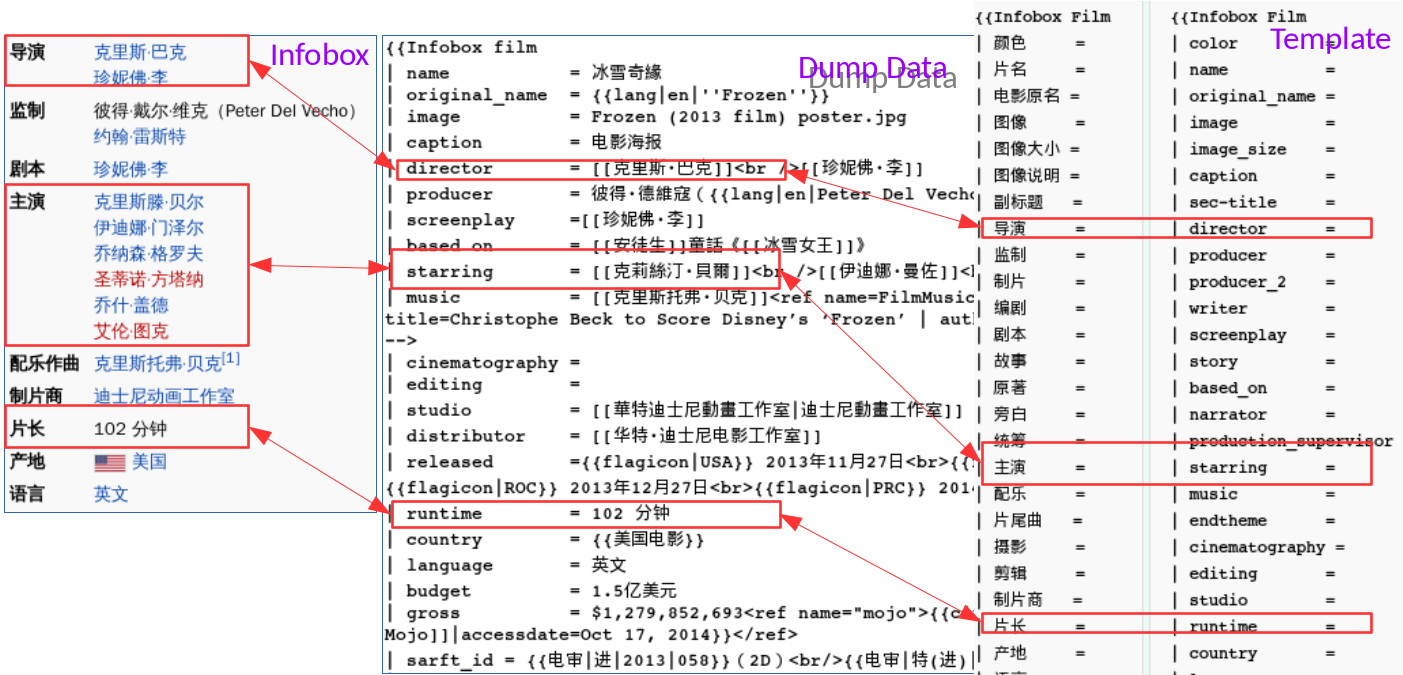
\includegraphics[width=1\columnwidth]{fig/infobox-template}}
        \caption{Comparison of display label and dump label in \emph{Interstellar} infobox}
        \label{fig:infobox-template}
    \end{figure}%
\item There are special characters in labels. Wikipedia usually use hyphen "-" or dot "•" to mark sublabels. For example, \emph{population} property has sub-properties "-Density" and "-Urban". In addition, odd signs, such as colon or asterisk, may occur in Baidu or Hudong property labels by mistake.
\end{itemize}

To solve the problems above, we take advantage of template information. Specifically, Wikipedia institutes rules of rendering label in templates. For example, movie infobox follows template \emph{Infobox film}, which is shown on the right of Fig.\ref{fig:infobox-template}, where both display labels and dump labels come from. When a dump label in triple-bracket occurs in dump file, we replace it by its mapping display label. After convert all the dump labels, we make a filter to redress the label text.

\subsection{Instance Extraction}
\label{sec:ie}
In encyclopedia, an article describes an unique entity in the world. Therefore we can extract an article content as an instance. During the extraction, illustrative or structure-related articles in Wikipedia are deleted, including category list pages and template documentations.

Each instance contains relations with concepts and properties. Take the movie 星际穿越(Interstellar) in Fig.\ref{fig:interstellar} as an example, concepts are assigned according to the category tags below the article page. 美国科幻片(American science fiction films) is a concept of Interstellar. In the meantime, we obtain label property from the article title and abstract property from the first paragraph. Infobox-properties are acquired via extracting from the infobox in the article. Besides, according to links in the content, we gain the reference $Li(a)$ between the current instance and others, such as 华纳兄弟(Warner Bros.).

After the preprocessing above, we harvest two types of information. One is the characteristics of instance, including $Ti(a)$, $Ab(a)$ of article$a$. The other includes relationships, containing $H^I$ and $H^P$ associated with article $a$.

\section{Cross-lingual Integration}
\label{sec:clkbb}
To construct a cross-lingual knowledge base with existing structured data, firstly we gather cross-lingual links which can help match the same entity in two languages and extend the link set. Secondly, we link this four encyclopedia, which is to say, respectively merging concepts, instances and properties from the four sources if they represent the same thing. Thirdly, we prune the taxonomy generated from concept relationships to retain a more accurate one. At last, we make instances and properties attached to the taxonomy to create a complete knowledge base.

\subsection{Cross-lingual Linking}
Wikipedia has \textcolor{red}{number} cross-lingual links between English and Chinese. By extracting language links from Wikipedia, we can get an initial cross-lingual link set of concepts and instances. Moreover, we utilize the language-independent method in \cite{wang2012cross} to extend the language-link set. With the linkage factor graph model, we harvest a cross-lingual links extension as many as 20 thousands with an ideal precision 85.5\% and a recall of 88.1\% between English Wikipedia and Baidu Baike.

However, due to following templates, Infobox-properties have no obvious cross-lingual links. To acquire such links, we take the following steps: (1) Given a matched template, which means $T_{e}$ and $T_{z}$ are cross-lingual pairs, find the display labels mapping the same dump label. That is to say, to two pairs, $p_{e}$ in $T_{e}$ and $p_{z}$ in $T_{z}$, if $tl_{e}$ is equal to $tl_{z}$, $<dl_{e},dl_{z}>$ are property cross-lingual; (2) Given the English and Chinese infoboxes of a matched instance, compare their templates, which are English template$T_{e}(a_{i})$ and a Chinese template$T_{z}(a_{j})$ in which $a_{i}$ and $a_{j}$ direct to the same entity, find the matched display labels mapping to the same dump label; (3) Given the English and Chinese infoboxes of a matched instance, to datatype properties, compare the similarity of literal value; to object properties, check whether the value refer to the same entity. 

In order to make all these encyclopedias linked to each other, we unify the same concept, instance and property from four sources, and give them unique identifiers. For instance, we merge instances by the following method:

\begin{enumerate}[Step 1]
    \item Given an instance extracted from Chinese Wikipedia, find the entity in Hudong and Baidu Baike with the same title.
    \item Given an instance extracted from Hudong, find the entity which is not in Chinese Wikipedia but in Baidu Baike with the same title.
    \item Other instances existing in only one encyclopedia are considered as independent instances. Up to now, we have combined all Chinese articles describing the same entity as one instance. Each instance may correspond to 1 to 3 sources.
    \item To a $L_{z}(a)$, find whether there is an English cross-lingual link in $CL<L_{e}, L_{z}>$. If exists, make the two as one instance and identify it using an ID.
    \item If a $L_{z}$ or a $L_{e}$ has no matched cross-lingual link, number it with an new ID.
\end{enumerate}

After the above steps, we acquire a list of instances and their unique IDs. Some of them contain cross-lingual information while some contain just monolingual information.

The process of unify concept and property is the same as instance. Meanwhile, all the relations in all sources are kept to prevent loss of information.

\subsection{Taxonomy Prune}
\label{sec:tp}
As a result of combining multi-source information without verifying, the taxonomy of concept system is mussy. For example, \textcolor{red}{example}. Therefore, we introduce the method from\cite{wang2014cross} to filter the correct SubClassOf and InstanceOf relations between two entities. Table. \ref{tab:} shows some examples of correct relations. In particular, some language-dependent literal and language-independent structural features are defined to vectorize each concept or instance. The literal features include the head words’ singular/plural forms of labels of English entities, the prefix/suffix relation of labels of Chinese entities. The structural features include article divergence for SubClassOf, property divergence for SubClassOf, category divergence for SubClassOf, article divergence for InstanceOf, property divergence for InstanceOf, category divergence for InstanceOf. By employing these features, a binary-classification model is trained based on Logistic Regression. The whole process is iterative by add assured result into training set and retraining the model to get higher precision. Confirming a right SubClassOf or InstanceOf not only depends on the prediction result of classification, but also cross-lingual knowledge validation, which ensures correctness if both the mapped English and Chinese relations are correct. 

The ideal result of pruning is a tree, whose edges, nodes, and leaves separately denote relations, concepts and instances. However, since getting rid of incorrect entity relations without consideration of integrity, a forest result is inevitable. We may omit some links but get more accurate relations instead.

\section{Result}
\label{sec:result}

\subsection{Extracted Knowledge Base}
We collect the resources from 4 wiki sites, English and Chinese Wikipedia dump files in 2015 April, Hudong html pages until 2014 May, and Baidu html pages until 2014 September. Each of the wikis has three types of information, which can be utilized for constructing our ontology, namely, specific articles, classification system, and attribute of articles. We extract each raw data, then form the extracted information into well-structured data. Table\ref{tab:extract-result} the result we get after elementary extraction in 4 different wiki sources.

\begin{table}[h]
\small
\centering
\caption{Statistics of elementary extraction result}
\label{tab:extract-result}
    \begin{tabular}{|l|l|l|l|l|}
        \hline
                 & Enwiki  & Zhwiki & Hudong  & Baidu   \\ \hline
        \#Instance & 4304113 & 662650 & 5590751 & 5622404 \\ \hline
        \#Concept  & 982432  & 159705 & 31802   & 1300    \\ \hline
        \#Property & 43976   & 18842  & 1187    & 139634  \\ \hline
    \end{tabular}
\end{table}

To build a knowledge base, we create URIs to identify each element and provide corresponding information if users look up elements over HTTP protocol to achieve the knowledge base. Table \ref{tab:uris} lists the defined URIs.
\begin{table}[h]
\small
\centering
\caption{URIs for concept, instance, property in our knowledge base}
\label{tab:uris}
    \begin{tabular}{|c|c|}
        \hline
        Type     & URI                          \\ \hline
        Concept  & http://xlore.org/concept/id  \\ \hline
        Instance & http://xlore.org/instance/id \\ \hline
        Property & http://xlore.org/property/id \\ \hline
    \end{tabular}
\end{table}

After fusing the heterogeneous resources, we harvest a cross-lingual graph with 1,093,855 classes, 200,223 properties, and 11,721,238 instances separately. With different methods of extraction and language linking discovery, these three kinds of entries show different results in languages. We give a breakdown of both Chinese knowledge and English knowledge in Table\ref{tab:kb-result}.

\begin{table}[h]
\small
\centering
\caption{Statistics of our knowledge base}
\label{tab:kb-result}
    \begin{tabular}{|l|l|l|l|}
        \hline
                        & Concepts  & Instance   & Property \\ \hline
        English         & 982,982   & 4,311,719  & 54,802   \\ \hline
        English\%       & 89.86\%   & 37.79\%    & 27.37\%  \\ \hline
        Chinese         & 176,648   & 7,842,117  & 167,083  \\ \hline
        Chinese\%       & 16.15\%   & 66.9\%     & 83.45\%  \\ \hline
        Cross-lingual   & 65,775    & 432,598    & 21,662   \\ \hline
        Cross-lingual\% & 6.01\%    & 3.7\%      & 10.82\%  \\ \hline
        Only English    & 917,207   &            & 33140    \\ \hline
        Only English\%  & 83.9\%    &            & 16.6\%   \\ \hline
        Only Chinese    & 110,873   &            & 145,421  \\ \hline
        Only Chinese\%  & 10.1\%    &            & 72.6\%   \\ \hline
        Sum             & 1,093,855 & 11,721,238 & 200,223  \\ \hline
    \end{tabular}
\end{table}

Our knowledge graph is organized in Openlink Virtuoso, which is a data management platform covering various server, including triple store. 

\subsection{Web Access to Knowledge Base}
We provide a website to present an intuitive graph of our knowledge in the forms of class, instance and property. Fig.\ref{fig:xlore} shows sample pages of the integrated data. The users of our system can choose language preference which is convenient for both English speaker and Chinese speaker. In the class webpage, we exhibit the label, super classes, subclasses, related topics, properties and instances of the specific class in bilingual way on condition that the corresponding English entries or Chinese entries exist.  In the instance webpage we display bilingual label, super classes, related classes, abstract, property key value pairs, images and references. In the property webpage, we presents bilingual label, domains, ranges, and related instances of each property. 
\begin{figure}[ht]
    \centerline{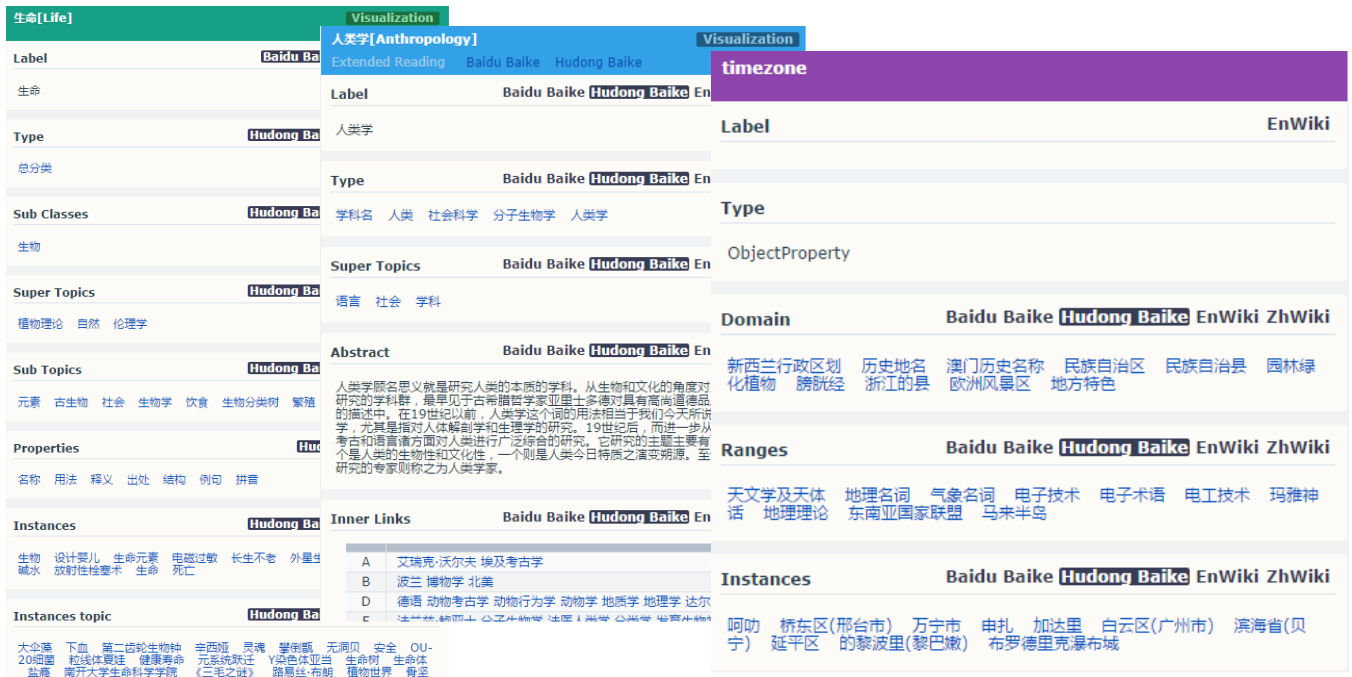
\includegraphics[width=1\columnwidth]{fig/xlore}}
    \caption{Sample Pages of Class, Instance and Property}
    \label{fig:xlore}
\end{figure}%
Beside these user-friendly pages, we provide two ways to access our knowledge base: via the search engine shown in Fig.\ref{fig:search-engine}, or via SPARQL endpoint shown in Fig.\ref{fig:sparql-endpoint}. For users who know little about semantic web, they can query by inputing related text into searchbox and search to get entities with similar label. To present practicable result, An index is generated over all entities. We as well provide SPARQL interface for professional users to query our knowledge graph. Users can choose the language tags of their desired results by \textbf{"filter(langMatches(?label),"en"))"} or \textbf{"filter(langMatches (?label),"zh"))"}.
%\begin{figure}
%    \centering
%    \begin{minipage}[t]{0.8\textwidth}
%        \centerline{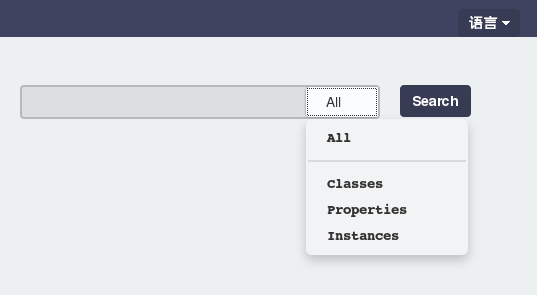
\includegraphics[width=0.8\columnwidth]{fig/search-engine}}
%        \caption{A Sample Query for Using Search Box }
%        \label{fig:search-engine}
%    \end{minipage}%
%    \begin{minipage}[t]{0.8\textwidth}
%        \centerline{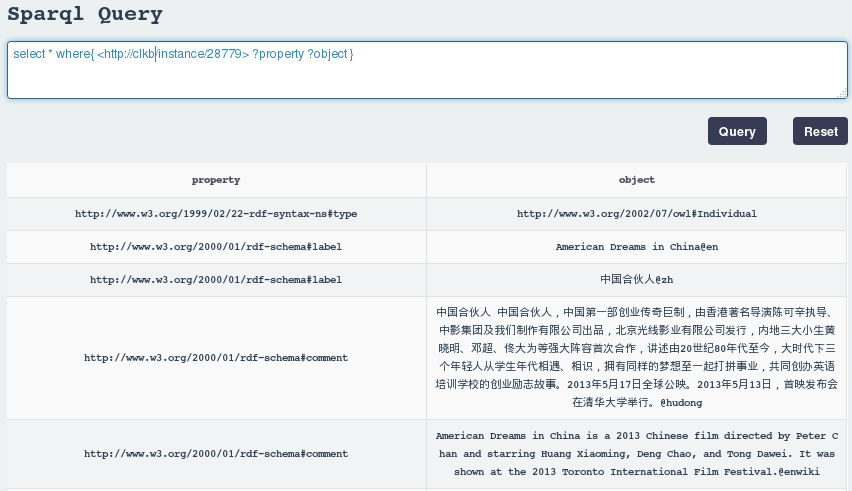
\includegraphics[width=0.8\columnwidth]{fig/sparql-endpoint}}
%        \caption{A SPARQL Sample Query over the Knowledge Base}
%        \label{fig:sparql-endpoint}
%    \end{minipage}%
%\end{figure}

\section{Related Work}
\label{sec:work}
In this section, we introduce some related knowledge bases and cross-lingual knowledge linking methods are referred to.
\subsection{Chinese Knowledge Bases}
Currently, several large-scale Chinese knowledge bases have been generated. Zhishi.me\cite{niu2011zhishi,wang2014publishing} is the first Chinese large-scale Linking Open Data published. It acquires structural information from three original sources, Chinese Wikipedia, Baidu Baike and Hudong Baike and gains more than 5 million distinct entities. Zhishi.me helps generate knowledge base focused on relations in Junfeng Pan’s work\cite{pan2012building}.
Similar with Zhishi.me, CKB\cite{wang2012building} is created from Hudong Baike. It first learns an ontology based on category system and properties, and then collects 19542 concepts, 2381 properties, 802593 instances. Besides using existing encyclopedias, CASIA-KB employs other types of sources(e.g. microblog posts, news pages, images) to enrich the structured knowledge.
\subsection{Cross-lingual Knowledge Bases}
DBpedia \cite{auer2007dbpedia,mendes2012dbpedia} is one of the most used cross-lingual knowledge base in the world. It's extracts various kinds of structured information from Wikipedia and employ the multilingual characteristic of Wikipedia to generate 97 language versions of content. This knowledge base is widely applied in many domains, including media recommendation \cite{passant2010dbrec,fernandez2011generic,kaminskas2012knowledge}, entity linking\cite{mendes2011evaluating} and information extraction \cite{dutta2013integrating}.
Universal WordNet(UWN)\cite{de2012uwn} is a large multilingual lexical knowledge base which is build from WordNet and enriched its entities from Wikipedia. It is constructed using sophisticated knowledge extraction, link prediction, information integration, and taxonomy induction methods. The API is available to over 200 languages and more than 16 million words and names. UWN provides semantic relationship of list of word meanings for Aya's work on conceptual search \cite{al2015conceptual}

%\subsection{Cross-lingual Knowledge Linking}
%Discovering more cross-lingual links is benefit to development of a multilingual knowledge base. General method is divided into two steps. First find missing link candidates using link structure of articles and then decide whether candidates are cross links or not by classification. \cite{sorg2008enriching} employs such approach to resolve the problem of automatically inducing new cross-language links. Wang\cite{wang2012cross} utilize a linkage factor graph model

\section{Conclusion}
\label{sec:con}
This paper presents a procedure of building a Chinese-English cross-lingual knowledge base from four encyclopedia sources. At first, data preprocessing work is done to extract structured information and unify data format. Then a cross-lingual lan-link set is generated to help combine the bilingual sources. Besides, an extension method is applied to enrich the links. To refine our dataset, we also do pruning work on taxonomy. Finally, we acquire a knowledge base containing XXX concepts, XXX instances and XXX properties. Currently, a SPARQL query interface is provided to access the knowledge base. 

%\section*{Acknowledgement}
%Thanks anonymous reviewers for their valuable suggestions that help us improve the quality of the paper. Thanks Prof. Chua Tat-Seng from National University of Singapore for discussion. The work is supported by 973 Program (No. 2014CB340504 ), NSFC-ANR (No. 61261130588), Tsinghua University Initiative Scientific Research Program (No. 20131089256) and THU-NUS NExT Co-Lab.

\bibliographystyle{splncs03}
\bibliography{paper}

%\end{CJK*}
\end{document}

